\section{Trees}
\emph{Connected acyclic graphs where two vertices are connected by only one path, with $|V| - 1$ edges in total.}

\subsection{Binary Search Trees}
\emph{A tree which is either empty or has \code{left} and \code{right} children binary trees.}

The \textbf{binary search tree property} states that all keys in the \code{left} sub-tree are less than the parent key,
and all keys in the \code{right} subtree are greater than the parent key.

The \textbf{height} of a BST is the number of edges on the longest path from the root to the leaf:\\[-0.2em]
\[ h(\code{v}) = \begin{cases} 
    0 & \text{if $v$ is a leaf} \\
    -1 & \text{if $v$ is null} \\
    \max(h(\code{v.left}), \; h(\code{v.right})) + 1 & \text{otherwise} \\
 \end{cases}
\]

The \textbf{minimum} and \textbf{maximum} keys are found by traversing the left and right subtrees respectively.

\textbf{Searching} for a specific key is done by comparing the key with the parent key,
recursively searching \code{v.left} if less than, \code{v.right} if greater than, and stopping if equal.

\textbf{Inserting} is akin to searching, but instead adding a new node at a leaf.

\textbf{Deleting} is trivial if if the node to be deleted has one or no children.
Otherwise, the node to be deleted is replaced by the minimum of the right subtree (its successor):

\begin{lstlisting}[
    mathescape,
    columns=fullflexible,
    basicstyle=\fontfamily{lmvtt}\selectfont,
  ]
successor(v):
    if v has a right child:
        return the minimum key in v.right
    else:
        walk up the tree to a node w
        where w.parent.left = w, or w is the root
        return w
\end{lstlisting}

All these operations are $O(h)$.
However, trees with the same keys need not have the same shape, and height depends on shape,
which is determined by insertion order.

There are $n!$ insertion orders, and $\approx 4^n$ possible shapes for a binary tree.

\subsection{AVL Trees}
\emph{Augmented BST which stores the tree height in each node.}

This augmented height field must be updated with every \code{insert} and \code{delete}.

A binary search tree is \textbf{balanced} iff $h = O(\log n)$, such that all operations take $O(\log n)$ time.

A node $v$ is \textbf{height-balanced} iff $|\code{v.left.height} - \code{v.right.height}| \leq 1$.
A height-balanced tree with $n$ nodes has height $h < 2 \log n$, and one with height $h$ has at least $n > 2^\frac{h}{2}$ nodes.

\subsubsection{Rotations}
\emph{Used to rebalance trees after insertion and deletion.\\ Left and right rotations are inverses of each other.}
\begin{center}
    \begin{forest}
        [$A_{k+2}$, red
            [$B_{k+1}$, baseline, blue
                [$L_{k}$, tier=0, roof]
                [$M_{k}$, tier=0, roof]
            ]
            [$R_{k-1}$, tier = 0, roof]
        ]
    \end{forest}
    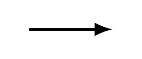
\begin{tikzpicture}
        \draw [-latex, very thick] (0,0) -- +(30pt,0);
        \end{tikzpicture}
    \begin{forest}
    [$B_{k+2}$, blue
        [$L_{k}$, tier=0, roof]
        [$A_{k+1}$, baseline, red
            [$M_{k}$, tier=0, roof]
            [$R_{k-1}$, tier=0, roof]
        ]
    ]
    \end{forest}
    \\[0.5em]Case 1: \textcolor{red}{$A$} is left-heavy but \textcolor{blue}{$B$} is balanced $\rightarrow$ right-rotate.

    \begin{forest}
        [$A_{k+2}$, red
            [$B_{k+1}$, baseline, blue
                [$L_{k}$, tier=0, roof]
                [$M_{k-1}$, tier=0, roof]
            ]
            [$R_{k-1}$, tier = 0, roof]
        ]
    \end{forest}
    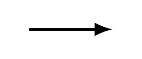
\begin{tikzpicture}
        \draw [-latex, very thick] (0,0) -- +(30pt,0);
        \end{tikzpicture}
    \begin{forest}
        [$B_{k+1}$, blue
            [$L_{k}$, tier=0, roof]
            [$A_{k}$, baseline, red
                [$M_{k-1}$, tier=0, roof]
                [$R_{k-1}$, tier=0, roof]
            ]
        ]
    \end{forest}
    \\[0.5em]Case 2: \textcolor{red}{$A$} is left-heavy but \textcolor{blue}{$B$} is left-heavy $\rightarrow$ right-rotate.

    \begin{forest}
        [$A_{k+2}$, red
            [$B_{k+1}$, baseline, tier=2, blue
                [$L_{k-1}$, roof, tier=1]
                [$C_{k}$, tier=1, magenta
                    [M1, roof]
                    [M2, roof]
                ]
            ]
            [$R_{k-1}$, roof, tier=1]
        ]
    \end{forest}
    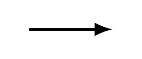
\begin{tikzpicture}
        \draw [-latex, very thick] (0,0) -- +(30pt,0);
        \end{tikzpicture}
    \begin{forest}
    [$A_{k+2}$, red
        [$C_{k+1}$, baseline, magenta
            [$B_{k}$, blue
                [$L_{k-1}$, roof, tier=0]
                [M1, roof]
            ]
            [M2, roof, tier=0]
        ]
        [$R_{k-1}$, roof, tier=0]
    ]
    \end{forest}
    \\[0.5em]Case 3: \textcolor{red}{$A$} is left-heavy but \textcolor{blue}{$B$} is right-heavy $\rightarrow$ left-rotate \textcolor{blue}{$B$},
    but \textcolor{red}{$A$} and \textcolor{magenta}{$C$} are still out of balance! M1 and M2 have a height of either $k-1$ or $k-2$.
\end{center}
\begin{center}
    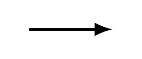
\begin{tikzpicture}
        \draw [-latex, very thick] (0,0) -- +(30pt,0);
    \end{tikzpicture}
    \begin{forest}
        [$C_{k+1}$, magenta
            [$B_{k}$, baseline, blue
                [$L_{k-1}$, roof, tier=1]
                [M1, roof, tier=0]
            ]
            [$A_{k}$, red
                [M2, roof, tier=0]
                [$R_{k-1}$, roof, tier=1]
            ]
        ]
    \end{forest}
    \\[0.5em]Case 3 (continued): Fixing the imbalance with a right-rotate about \textcolor{red}{$A$}.
\end{center}

After an \code{insert}, at most 2 rotations are needed, but \code{delete} may require up to $O(\log n)$ rotations.

This is because \code{delete} reduces height and rotations reduce height, so it is not sufficient to only fix
the lowest imbalanced node in the tree.

\subsection{Dynamic Order Statistics}
\emph{A tree data structure supporting not only insertion and deletion, but also selecting the k-th element.}

Augment a balanced tree with \textbf{weight} information $w$ on each node (not rank!):\\[-0.2em]
\[ w(\code{v}) = \begin{cases} 
    0 & \text{if $v$ is a leaf} \\
    w(\code{v.left}), \; w(\code{v.right}) + 1 & \text{otherwise} \\
 \end{cases}
\]

\begin{lstlisting}[
    mathescape,
    columns=fullflexible,
    basicstyle=\fontfamily{lmvtt}\selectfont,
  ]
select(k):
    rank = v.left.weight + 1
    if k = rank: return v;
    elif k < rank: return v.left.select(k)
    else k > rank: return v.right.select(k - rank)

rank(v):
    rank = v.left.weight + 1
    while v is not null:
        if v is left child: do nothing
        else: rank += v.parent.left.weight + 1
        v = v.parent
    return rank
\end{lstlisting}

Weights need to be updated with every rotation caused by \code{insert} and \code{delete}.

\subsection{Dictionary}
\emph{An abstract data type akin to a symbol table, but with support for successor and predecessor queries.}

Implemented with balanced trees.

\subsection{Interval Trees}
\emph{A binary tree data structure where every node is an interval, and the tree is ordered by the lower bound of the interval.}

We will need to augment each node with the \textbf{maximum upper bound} of the intervals in both subtrees,
and also update this after every rotation.

\begin{lstlisting}[
    mathescape,
    columns=fullflexible,
    basicstyle=\fontfamily{lmvtt}\selectfont,
  ]
interval_search(x):
    while c is not null and x is not in c.interval:
        if c.left is null: c = c.right
        elif x > c.left.max: c = c.right
        else c = c.left
    return c.interval

all_overlaps(x):
    repeat until no more intervals:
        interval = interval_search(x)
        add interval to list
        delete interval from tree
    add all intervals back to tree
\end{lstlisting}

\code{interval-search} takes $O(\log n)$ time, and \code{all-overlaps} takes $O(k \log n)$ time.

\subsection{Range Trees}
\emph{A binary tree data structure supporting orthogoanl range searching to determine the number of points within a range.}

Unlike regular trees, range trees store points only in the leaves, and internal nodes store the largest value of its left subtree.

\begin{lstlisting}[
    mathescape,
    columns=fullflexible,
    basicstyle=\fontfamily{lmvtt}\selectfont,
  ]
find_split(lo, hi):
    v = root
    loop:
        if hi $\leq$ v.key: v = v.left
        elif lo > v.key: v = v.right
        else: break
    return v
\end{lstlisting}

For a 1D range query, once the split node is found with \code{find-split},
we traverse both the left and right subtrees as long as they are within the \code{lo-hi} range.

An invariant is that the search interval for a left-traversal at node $v$ includes the maximum item in the subtree rooted at $v$.

This takes $O(k + \log n)$ time, where $k$ is the number of points found.
However, it takes $O(n \log n)$ time to pre-process (build) the tree, and $O(n)$ space.

If we instead only wanted to know the number of points within a range,
we only need to augment the tree with the number of nodes in each subtree rather
than traversing entire subtrees.

This generalizes to $d$-dimensions by storing a $d-1$-dimensional range tree in each node
of a 1D range tree and constructing the $d-1$-dimensional range tree recursively.

However, rotations take $O(n)$, so we don't support \code{insert} and \code{delete}.
In general, queries take $O(\log^d n + k)$, building the tree takes $O(n \log^{d-1} n)$, and
the tree takes $O(n \log^{d-1} n)$ space.

\subsection{(a, b) Trees}
The value for $a$ is constrained: $2 \leq a \leq \frac{b + 1}{2}$.

Nodes in $(a, b)$-trees can store \textbf{multiple keys}, where $a - 1 \leq n_{\text{keys}} \leq b - 1$, with the exception
of the root node which may have 1 key at minimum.

Therefore, internal nodes have between $a$ and $b$ children inclusive, leaf nodes have none, and the root node can have
at least 2 and at most $b$ children.

We can see that every non-leaf node must have one more child than its number of keys.
These keys must be in sorted ascending order, and form a \textbf{key range}.

For a non-leaf node with $k$ keys $v_1, v_2, \dots v_k$ and $k + 1$ children $t_1, t_2, \dots t_{k+1}$:

$\forall v \in t_1, \; v \leq v_1$ \\
$\forall v \in t_{k+1}, \; v > v_k$ \\
$\forall i \in [2, k], \; \forall v \in t_i, \; v \in (v_{i-1}, v_i]$

Additionally, all leaf nodes must be at the same depth.

\textbf{B-trees} are simply $(B, 2B)$-trees.

\code{search} is trivial: descend through sub-trees by comparing the key with the node's key range.

\code{insert} is trivial unless there is an overflow, in which case we \code{split} the node and insert the new key.

\code{split} takes the median key in a node and conjoins it with its parent, and the keys to the left and right
of the median key become its children. The parent might overflow, and if so we \code{split} it again, and so on.

\code{delete} swaps the node to be deleted with its predecessor's or successor's leaf, before deleting.
Then, the leaf node may become underfull. If the sibling can donate one key, we move the parent's key
down and the sibling's key up. Otherwise, we \code{merge} both siblings.

\code{merge} moves the parent down between the two children and conjoins all of them into one node.
The parent might become underfull, and if so we \code{merge} its parent, and so on.

All operations take $O(\log n)$ time.